%%%%%%
%
% $Autor: Wings $
% $Datum: 2020-01-18 11:15:45Z $
% $Pfad: githubtemplate/Template/Presentations/Template/slides/rename.tex $
% $Version: 4620 $
%
%
% !TeX encoding = utf8
% !TeX root = Rename
%
%%%%%%



%\Mysection{Anforderung}

\STANDARD{Bauteilskizze}
{ 
	
  \framesubtitle{Was ist das Produktziel}	
 

  \begin{itemize}
    \item \textbf{Anwenderziel:} Demonstrationsmodell eines geregelten elektrischen Tischförderbandes mit DC-Motor 
    \item \textbf{Hauptfunktion:} Transport von Kleinbauteilen (Faustgroß)
    
\end{itemize}
}

\STANDARD{Verbauskizze}
{ 
	
	\framesubtitle{Was ist das Produktziel}	
	
	
	\begin{itemize}
		\item \textbf{Anwenderziel:} Demonstrationsmodell eines geregelten elektrischen Tischförderbandes mit DC-Motor 
		\item \textbf{Hauptfunktion:} Transport von Kleinbauteilen (Faustgroß)
		
	\end{itemize}
}

\STANDARD{Technische Daten}
{ 
  \textbf{Anforderungen}:\\
  Transport von Kleinbauteilen, Regeln auf Zielgeschwindigkeit.\\ 
  Erfassung  eines Objektes am Anfang und am Ende des Förderbandes im Automatikmodus 

  
} 

\STANDARD{Beschreibung}
{ 
	\textbf{Anforderungen}:\\
	Transport von Kleinbauteilen, Regeln auf Zielgeschwindigkeit.\\ 
	Erfassung  eines Objektes am Anfang und am Ende des Förderbandes im Automatikmodus 
	
} 

\STANDARD{Aufgaben im System}
{ 
	\textbf{Anforderungen}:\\
	Transport von Kleinbauteilen, Regeln auf Zielgeschwindigkeit.\\ 
	Erfassung  eines Objektes am Anfang und am Ende des Förderbandes im Automatikmodus 


} 
\STANDARD{Aufgaben im System}
{ 
	\textbf{Anforderungen}:\\
	Transport von Kleinbauteilen, Regeln auf Zielgeschwindigkeit.\\ 
	Erfassung  eines Objektes am Anfang und am Ende des Förderbandes im Automatikmodus 
	
	
} 
\STANDARD{Aufgaben im System}
{ 
	\textbf{Anforderungen}:\\
	Transport von Kleinbauteilen, Regeln auf Zielgeschwindigkeit.\\ 
	Erfassung  eines Objektes am Anfang und am Ende des Förderbandes im Automatikmodus 
	

} 


%\STANDARD{Konzeptskizze}
%{ 
%+	
%	\begin{figure}
%		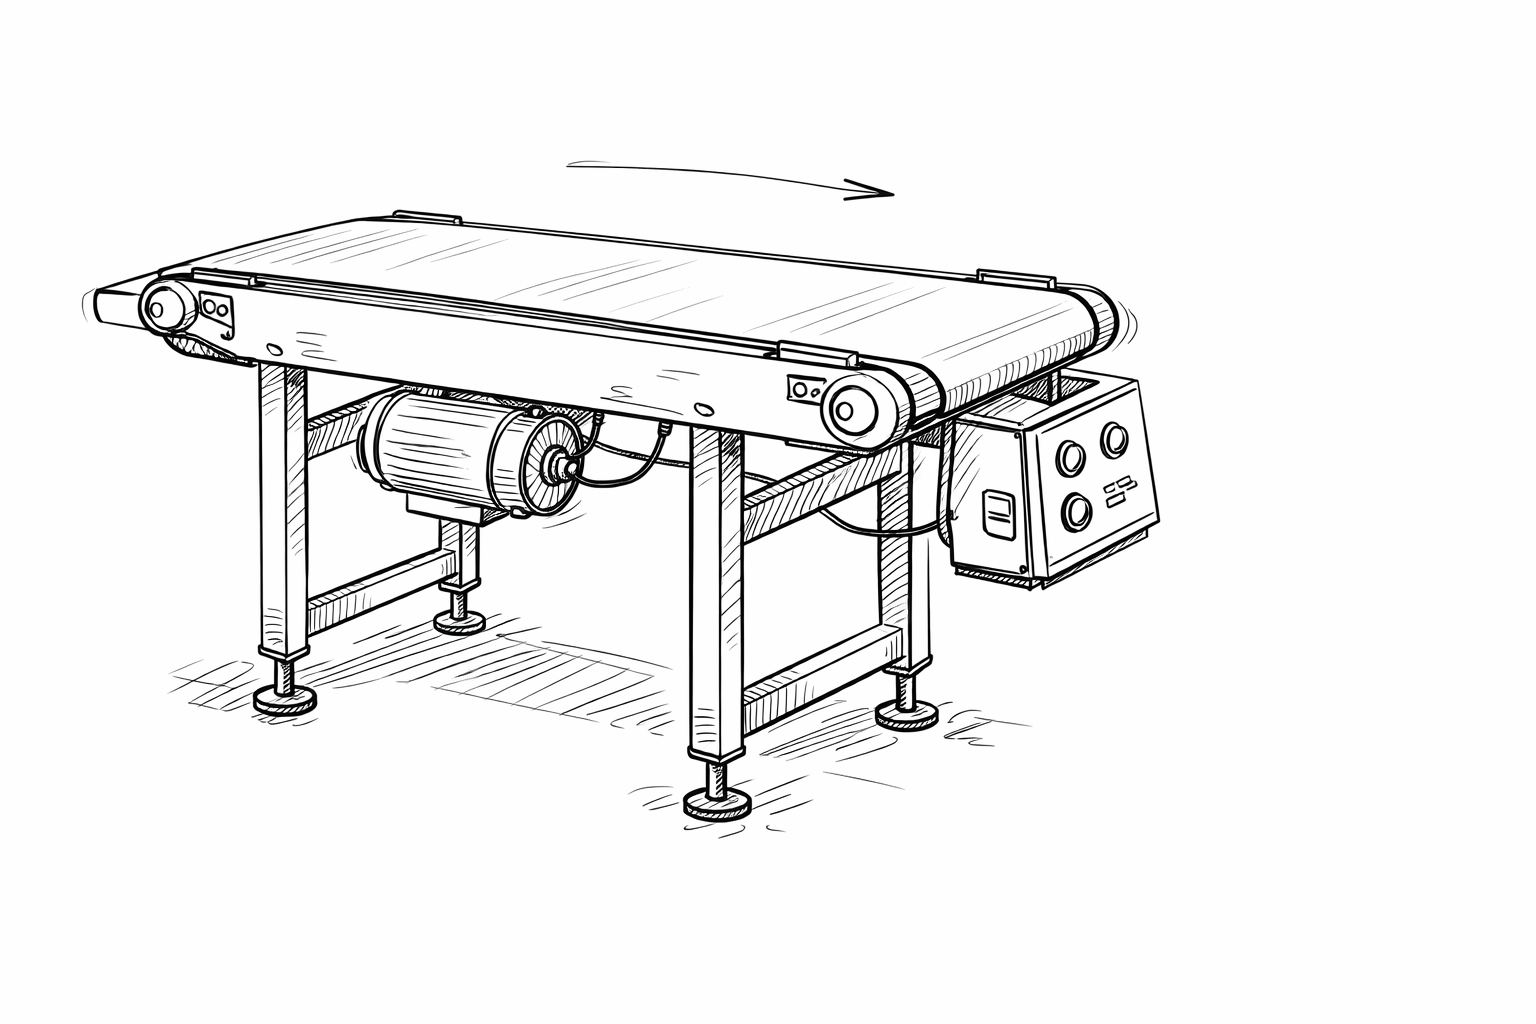
\includegraphics[width=\textwidth]{img/ConveyorSketch}
%	\end{figure}
%} 




